% !TEX TS-program = xelatex
% !TeX spellcheck = ru_RU

\documentclass{article}

\usepackage{hyperref}
\usepackage{polyglossia}
\setmainlanguage{russian}
\setotherlanguage{english}
\usepackage{csquotes}
\pagenumbering{gobble}
\usepackage[a5paper]{geometry}
\geometry
  {top=18pt
  , bottom=14pt
  ,left=.5cm,right=1cm
  }

\setmainfont[Ligatures=TeX]{Liberation Serif}
\setsansfont[Ligatures=TeX]{Liberation Sans}
\setmonofont[Scale=1.0,
BoldFont=lmmonolt10-bold.otf,
ItalicFont=lmmono10-italic.otf,
BoldItalicFont=lmmonoproplt10-boldoblique.otf
]{lmmono9-regular.otf}

\usepackage{graphicx}
\def\worktitle{Машинное обучение с помощью автоматического порождения текстов учебных практик}
\title{Отзыв научного руководителя о прохождении  учебной практики \enquote{\worktitle}}

\date{\today}
\def\Jsoo{\textsc{Js\_of\_ocaml}}
\def\Javascript{\textsc{Javascript}}
\def\OCaml{\textsc{OCaml}}

\begin{document}
\maketitle
В ходе  учебной  практики \textit{Колесов Сан Сарыч} разрабатывал инструмент,
который путём обучения на текстах учебных практик студентов математико-механического факультета,
достигает сильного искусственного интеллекта.
Это является актуальной задачей особенно для матмеха, так как средний уровень обучающихся постоянно падает, близок к нулю и скоро переполнит целочисленный тип \verb=uint8_t=.

В ходе учебной практики защищающий \textbf{(не)качественно} выполнял поставленные задачи,
\textbf{(не)своевременно} общался с руководителем и
\textbf{(не)проявлял} самостоятельность.
В том числе защищающийся {\small (перечисление задач)}
\begin{itemize}
\item Ограбил  1 корован.
\item Патчил KDE 2 под FreeBSD.
\item Решал 1 неразрешимую задачу.
\end{itemize}

\noindent В ходе работы Защищающийся изучил и применил следующие технологии: (чему обучающийся научился в ходе практики).

Считаю, что Отличников С. С. за учебную практику заслуживает \enquote{\textbf{зачёт (ECTS A-E)}} / \enquote{\textbf{незачёт (ECTS F)}}.

\vspace{1cm}
\begin{figure}[!htb]
    \centering
    \begin{minipage}{.4\textwidth}
        \centering
     старший преподаватель кафедры системного программирования Пушкин~А.~С.
    \end{minipage}%
    \begin{minipage}{0.58\textwidth}
    \begin{flushright}
     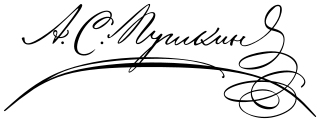
\includegraphics[width=.9\linewidth]{signature.png}\\
     % picture from
     % https://upload.wikimedia.org/wikipedia/commons/thumb/9/90/%D0%9F%D1%83%D1%88%D0%BA%D0%B8%D0%BD_%D0%90%D0%BB%D0%B5%D0%BA%D1%81%D0%B0%D0%BD%D0%B4%D1%80_%D0%B0%D0%B2%D1%82%D0%BE%D0%B3%D1%80%D0%B0%D1%84.svg/320px-%D0%9F%D1%83%D1%88%D0%BA%D0%B8%D0%BD_%D0%90%D0%BB%D0%B5%D0%BA%D1%81%D0%B0%D0%BD%D0%B4%D1%80_%D0%B0%D0%B2%D1%82%D0%BE%D0%B3%D1%80%D0%B0%D1%84.svg.png
    \end{flushright}
    \end{minipage}
\end{figure}

\end{document}
